\documentclass{beamer}
%Les packages pour écrire des math
\usepackage{amsmath}
\usepackage{amsthm}
\usepackage{amssymb}
\usepackage{mathabx}
\usepackage{dsfont} %Fonction caractéristique
\usepackage{stmaryrd}
\numberwithin{equation}{section}

\usepackage{listings}
\usepackage[authoryear]{natbib}



\usepackage{hyperref}
\usepackage{url}

\usepackage{algorithm}
\usepackage{algorithmic}

%\usepackage[francais]{babel}	
\usepackage[utf8]{inputenc}
%\usepackage[T1]{fontenc}

\usepackage{graphicx}
\usepackage{multicol}
%\usepackage{pst-solides3d}
\graphicspath{ {./images/} }
\usepackage[font=small,labelfont=bf]{caption}
\usepackage{subcaption}

%Information to be included in the title page:
\titlegraphic{\parbox[c]{3cm}{
\includegraphics[scale=0.18]{emse.png}}\hspace*{1cm} \parbox[c]{3cm}{
\includegraphics[scale=0.33]{LSCE.jpg}}}
\title{Changement d’échelles dans les projections climatiques et leurs impacts hydrologiques: Cas des grandes plaines américaines}
\author{Mathis Deronzier}
\date{Septembre 2021}

\begin{document}
	\frame{\titlepage}
	
	\begin{frame}{Introduction}
		\begin{minipage}[b]{1\linewidth}{Des changements climatiques majeurs au cours de ces prochaines années}
			\begin{figure}
				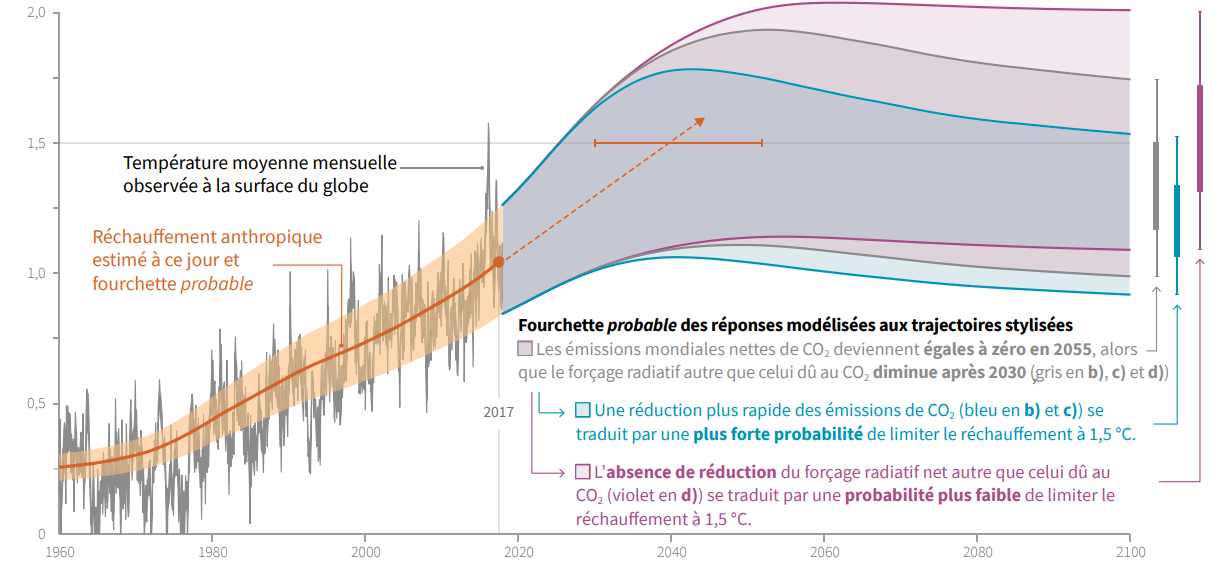
\includegraphics[scale=0.25]{proj_GIEC.png}
				\caption{Réchauffement planétaire par rapport à la période $1850-1900 (^{\circ}C)$}
			\end{figure}
		\end{minipage}
	\end{frame}
	
	\begin{frame}{Les enjeux de ce stage}
		\begin{block}{Les problématiques de ce stage:}
			\begin{itemize}
				\item Comment utiliser des modèles climatiques Globaux pour anticiper des modifications locales du climat?
				\item Dans quelle mesure les modèles de climats respectent-ils les lois de la physique?
				\item Quel est l'impact des différentes échelles sur les prévisions climatiques?
			\end{itemize}
		\end{block}
		\begin{block}{Les points étudiés durant ce stage:}
			\begin{itemize}
				\item Les modèles Hydrologiques
				\item Les méthodes de downscaling
				\item Les problématiques d'upscaling
				\item La modélisation hydrologique du Little Washita
			\end{itemize}
		\end{block}
	\end{frame}
	\begin{frame}{Sommaire}
		\tableofcontents
	\end{frame}

	\section{Modèles de climat et modélisation hydrologique}	
	\subsection{Les modèles de climat}
	\begin{frame}
	\begin{block}{Interactions climatiques}
	\begin{figure}[H]
		\begin{center}
			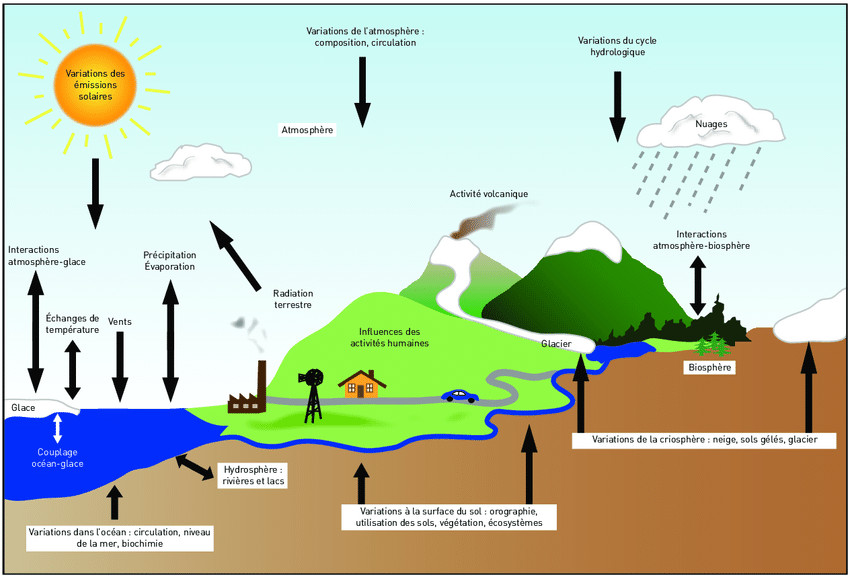
\includegraphics[scale=0.18]{images/interaction_climat.png}
		\end{center}
	\end{figure} 
	\end{block}
	\begin{block}{Modélisation des interactions}
		\begin{figure}
		\begin{center}
			\begin{subfigure}[b]{0.45\textwidth}
				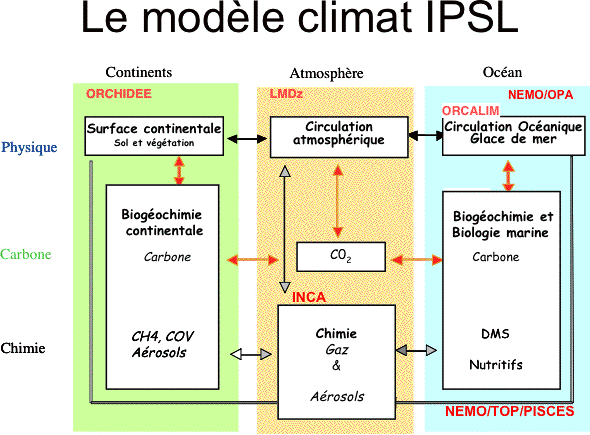
\includegraphics[scale=0.19]{images/modele_climat_IPSL.png}
			\end{subfigure}
			\hfill
			\begin{subfigure}[b]{0.45\textwidth}
				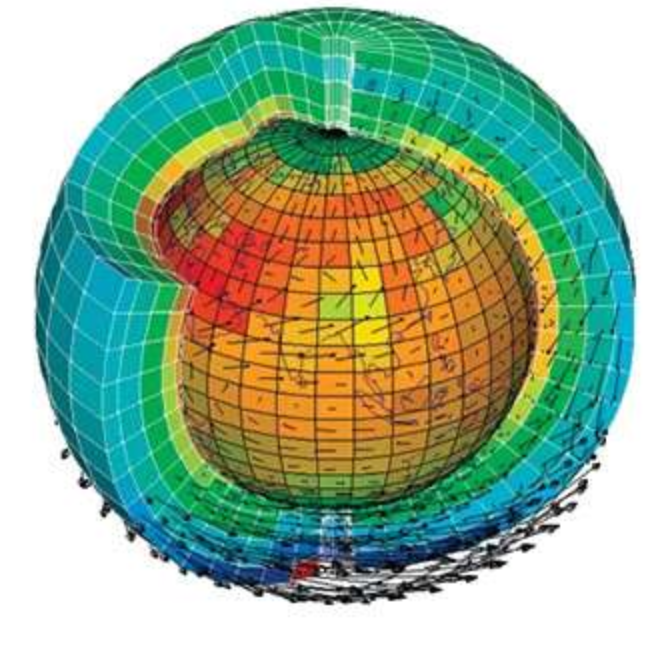
\includegraphics[scale=0.13]{images/maillage_terre.png}
			\end{subfigure}
		\end{center}
		\end{figure}
	\end{block}
	\end{frame}

	\subsection{Les interaction sol-atmosphère}
	
	\subsubsection{Les précipitations}
	
	\begin{frame}{L'eau entrante dans le sol}
		\begin{block}{Précipitations dans les modèle hydrologique}
			\begin{itemize}
				\item Définition: eau tombant sur la terre sous toutes ses formes (pluie, neige, grésil, grêle)
				\item Origine: Condensation liée à un changement de température ou de pression 
			\end{itemize}
		\end{block}
		\begin{block}{Types de précipitations}
			\begin{itemize}
				\item Précipitations convectives
				\item Précipitation orographiques
				\item Précipitation frontales 
			\end{itemize}
		\end{block}
	\end{frame}

	\subsubsection{L'évapotranspiration}
	
	\begin{frame}{Les mécanismes d'eau sortante du sol}
		\begin{minipage}[b]{0.5\linewidth}
			\begin{figure}
				\begin{center}
					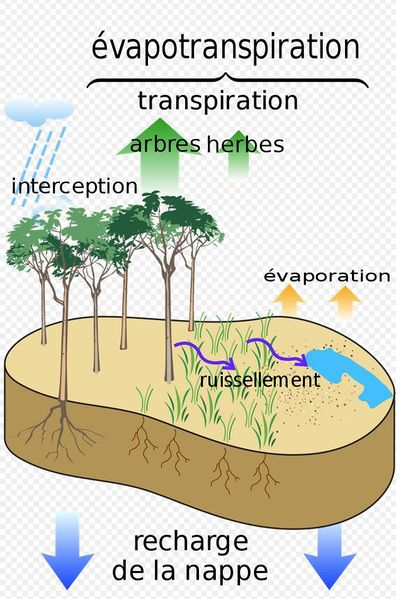
\includegraphics[scale=0.35]{images/evapotranspiration.jpg}
				\end{center}
			\caption{L'évapotranspiration}
			\end{figure} 
		\end{minipage}\hfill
		\begin{minipage}[b]{0.5\linewidth}
					\begin{figure}
						\begin{center}
							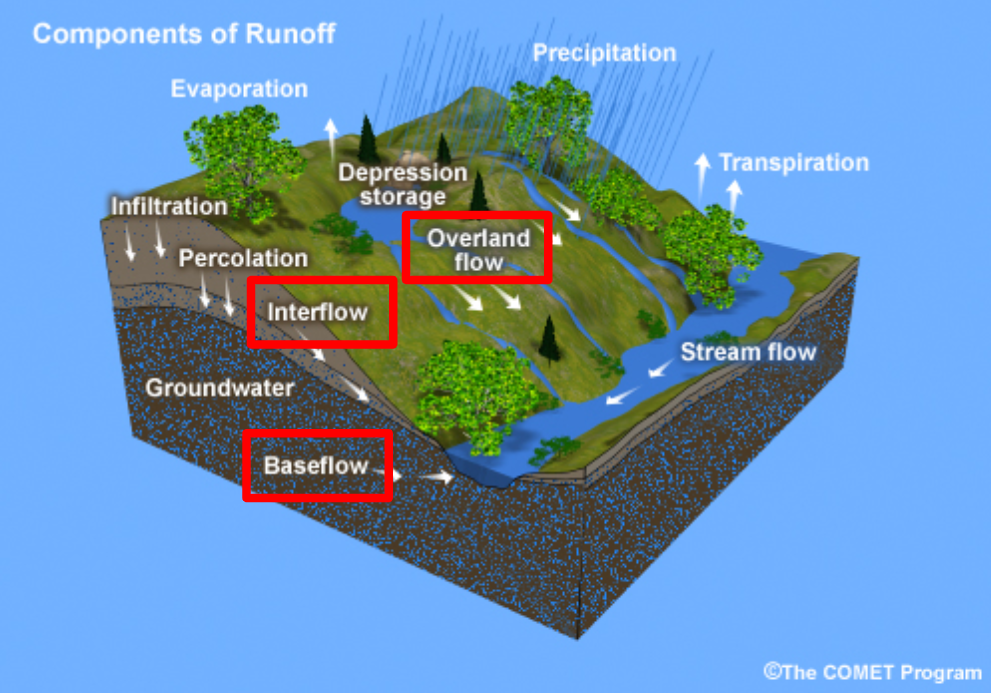
\includegraphics[scale=0.18]{different_flows.png}
						\end{center}
					\caption{Les mécanismes des écoulements}
					\end{figure} 
		\end{minipage}
	\end{frame}

	\subsubsection{Bilan hydrique}
	
	\begin{frame}{Les mécanismes d'eau sortante du sol}
		\begin{minipage}[b]{0.5\linewidth}
			\begin{figure}
				\begin{center}
					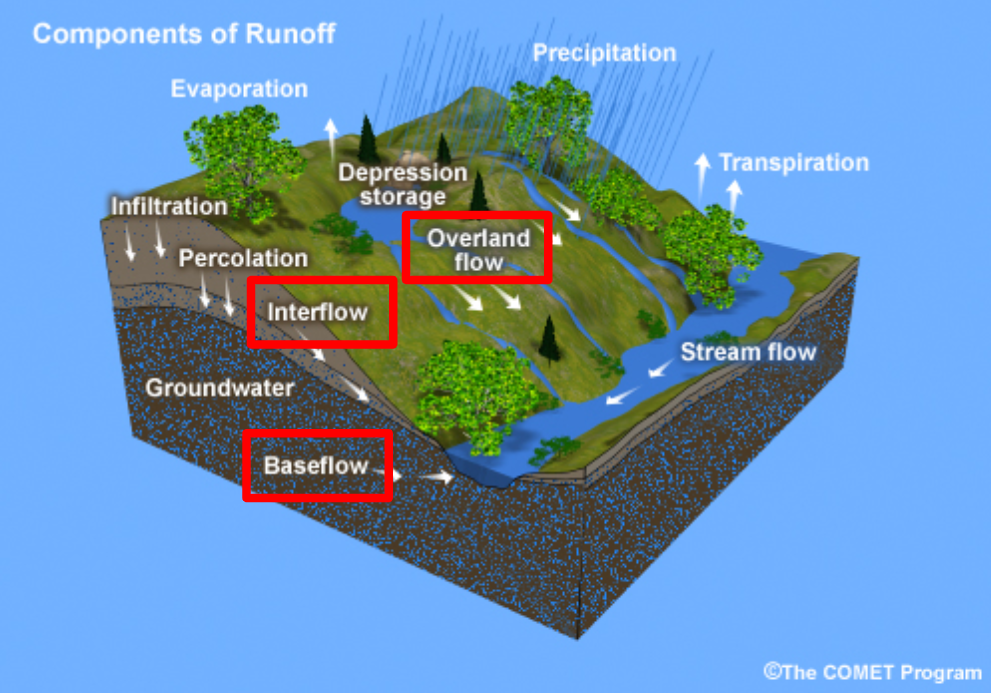
\includegraphics[scale=0.13]{different_flows.png}
				\end{center}
				\caption{L'évapotranspiration}
			\end{figure} 
		\end{minipage}\hfill
		\begin{minipage}[b]{0.5\linewidth}
			\begin{block}{Équations milieu poreux}
			Équation de conservation de la masse:
			\begin{equation}
				\label{eq-mass-por}
				div(\overrightarrow{U})+\frac{\partial}{\partial t}(\theta)+ q=0.
			\end{equation}
			Équation de Darcy:
			\begin{equation}
				\label{eq-Darcy}
				\overrightarrow{U}=\frac{k}{\mu }(\overrightarrow{\nabla}\, p+\rho g \,\overrightarrow{\nabla}\, z).
			\end{equation} 
			Équation de Richards:
			\begin{equation}
				\label{eq-rapp-dens-H}
				S_s(H)\frac{\partial H}{\partial t}=\frac{\partial\theta}{\partial t}.
			\end{equation}
			\end{block}
		\end{minipage}
	\end{frame}
	
	\section{Modélisation hydrologique du Little Washita}
	
	\begin{frame}{Méthodologie pour les modélisations hydrologiques}
			\begin{figure}
				\begin{center}
					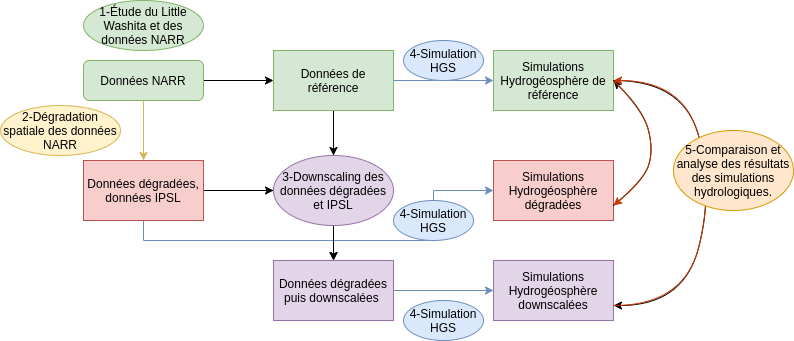
\includegraphics[scale=0.4]{Diagrame_methodo.png}
				\end{center}
				\caption{Diagramme de la méthodologie utilisée pour le stage}
			\end{figure} 
	\end{frame}
	
	\subsection{Le little Washita}
	
	\begin{frame}{Le Little Washita}
		\begin{minipage}[b]{0.6\linewidth}
			\begin{figure}
				\begin{center}
					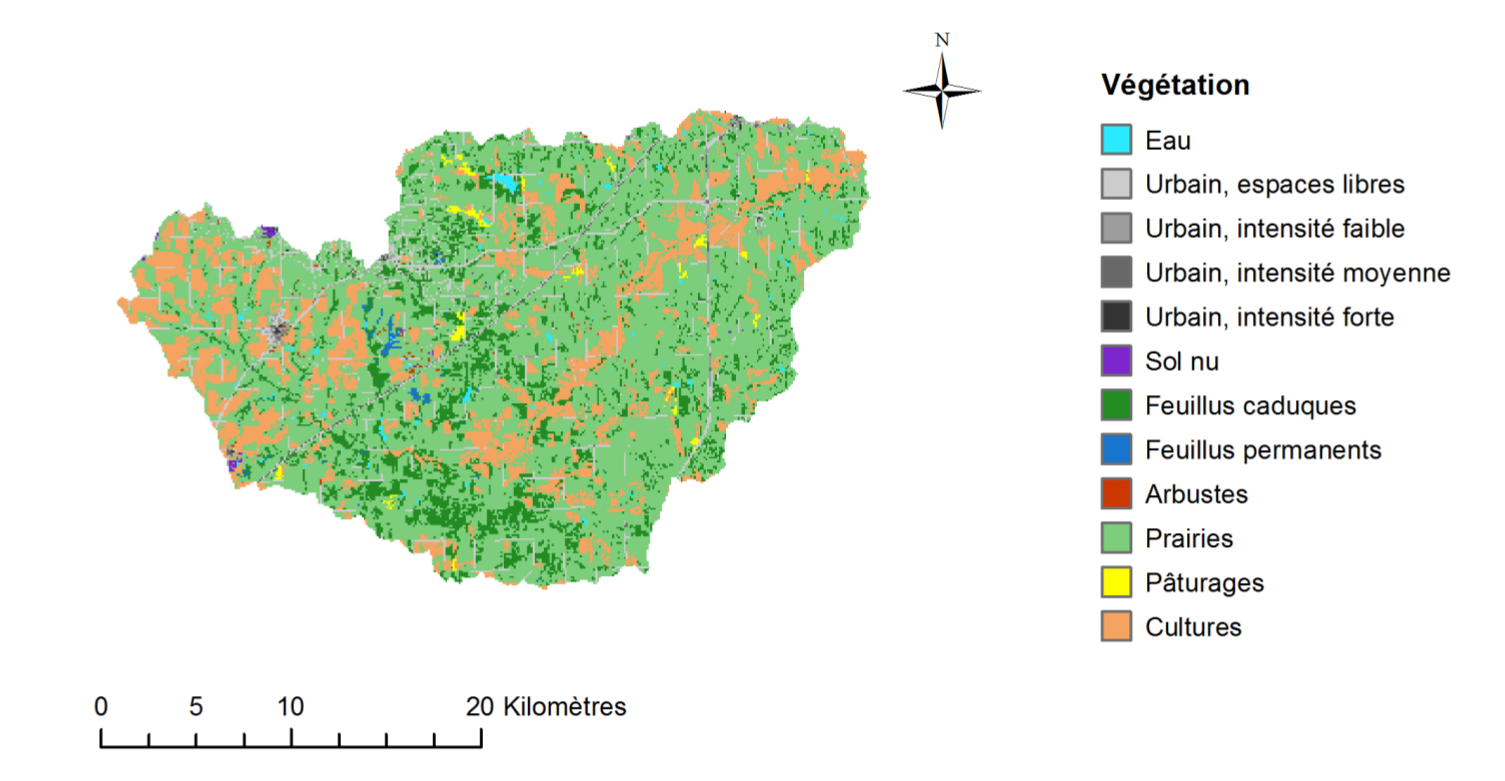
\includegraphics[scale=0.12]{little_washita_vegetation.png}
				\end{center}
				\caption{L'évapotranspiration}
			\end{figure} 
		\end{minipage}\hfill
		\begin{minipage}[b]{0.4\linewidth}
			\begin{block}{Caractéristiques du Little Washita}
				\begin{itemize}
					\item Surface: 611 $km^2$
					\item Climat: continentale tempérée
					\item Altitude: $320-474m$
					\item Pentes: moyenne ($3.4\%$), maximale ($12\%$)
				\end{itemize}
			\end{block}
		\end{minipage}
	\end{frame}
	\subsection{Les données NARR et IPSL}
	\begin{frame}{Les données North American Regional Realanalysis et IPSL}
		\begin{minipage}[b]{0.5\linewidth}
			\begin{figure}[H]
				\begin{center}
					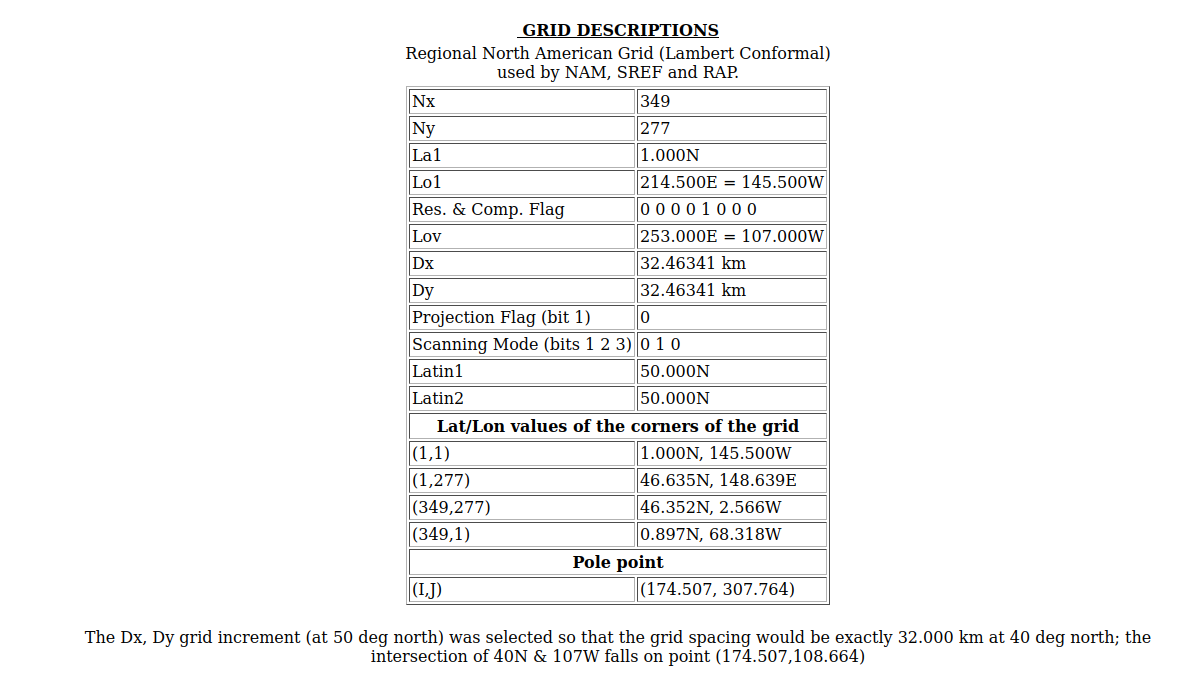
\includegraphics[scale=0.12]{grid_prop.png}
				\end{center}
				\captionof{figure}{Description du maillage NARR}
				\label{fig-maillage NARR}
			\end{figure}
		\end{minipage}\hfill
		\begin{minipage}[b]{0.5\linewidth}
			\begin{figure}[H]
				\label{fig-proj Lambert}
				\begin{center}
					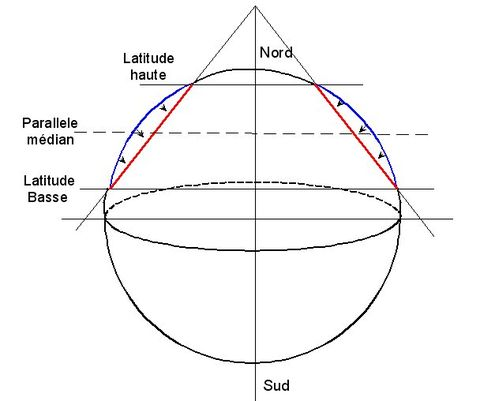
\includegraphics[scale=0.3]{lambert.jpg}
				\end{center}
				\caption{Projection conique conforme de Lambert}
			\end{figure}
		\end{minipage}	
	\end{frame}
	
	\subsection{La dégradation des données}
	\begin{frame}{Les données North American Regional Realanalysis et IPSL}
		\begin{figure}[H]
			\begin{center}
				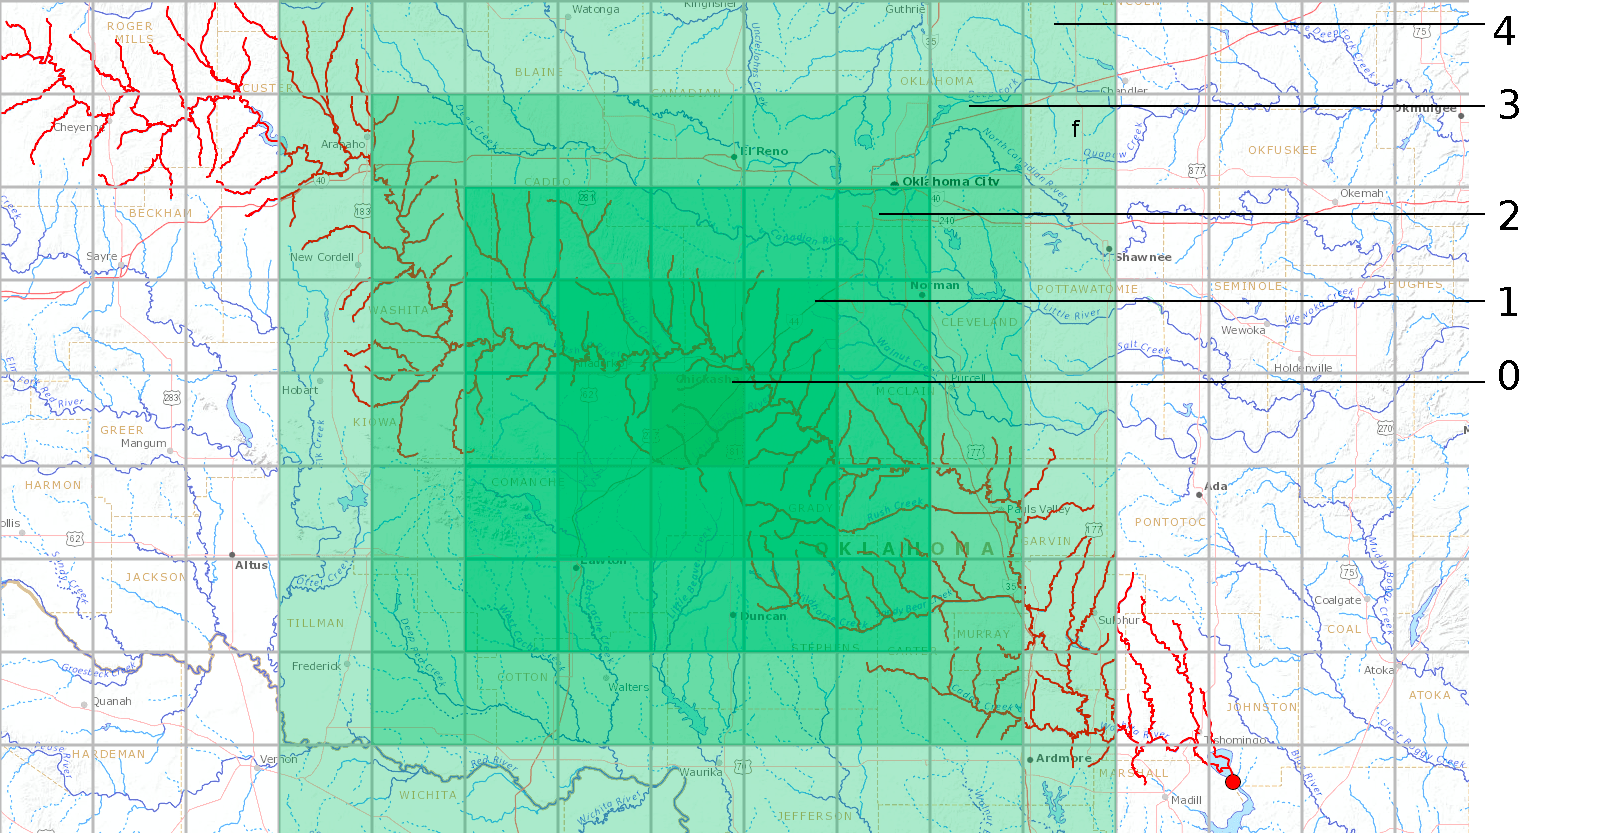
\includegraphics[scale=0.2]{Little_Washita_deg.png}
			\end{center}
			\captionof{figure}{Les différentes zones de dégradation considérées pour le Little Washita}
			\label{fig-Little-Washita-deg}
		\end{figure}
	\end{frame}
	\subsection{Downscaling des données}
	
	\subsubsection{Méthode de downscaling}
	\begin{frame}{Méthode de downscaling}
		\begin{minipage}[b]{0.5\linewidth}
			\begin{block}{Résultat du downscaling des données}
				\begin{itemize}
					\item $X=X_1,X_2,...,X_n$ et $X'=X'_1,X'_2,...,X'_m$ les réalisations des données downscalées passées et futures
					\item $Y=Y_1,Y_2,...,Y_n$ et $Y'=Y'_1,Y'_2,...,Y'_m$ les réalisations des données réelle passées et futures
					\item $\mathcal{F}_{X}$ et $\mathcal{F}_{Y}$ les fonctions de répartitions empriques 
				\end{itemize} 
			\end{block}
		\end{minipage}\hfill
		\begin{minipage}[b]{0.4\linewidth}
			\begin{block}{Exemple du downscaling avec l'algorithme }
				-Image représentative du downscaling
			\end{block}
		\end{minipage}
	\end{frame}

	\subsubsection{Résultats du downscaling des données}

	\begin{frame}{Analyses des résultats du downscaling}
		\begin{minipage}[b]{0.5\linewidth}
			\begin{figure}
				\label{fig-res_CVM_CDFt}
				\centering
				\begin{subfigure}[b]{0.5\textwidth}
					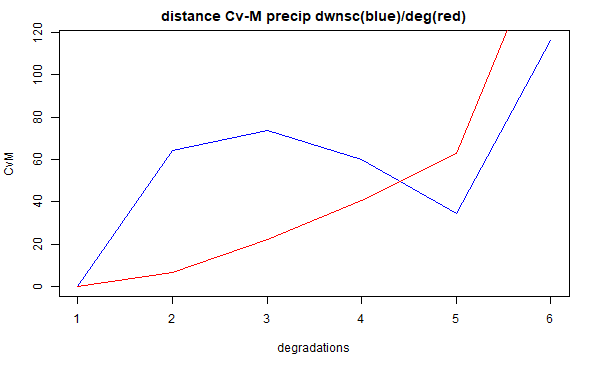
\includegraphics[scale=0.2]{images/Dist_CVM_precip_CDFt.png}
				\end{subfigure}\\
				\begin{subfigure}[b]{0.5\textwidth}
					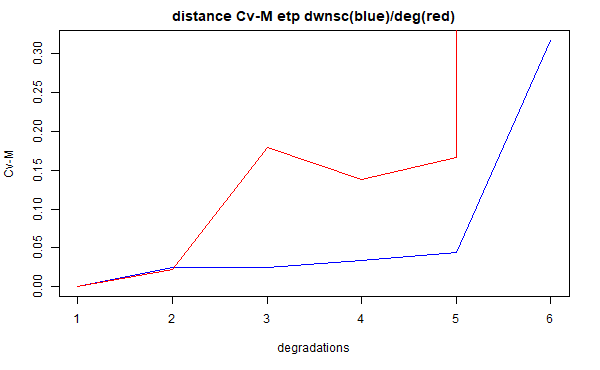
\includegraphics[scale=0.2]{images/Dist_CVM_evap_CDFt.png}
				\end{subfigure}
				\caption{Tracé de la distance de Cramér-von Mises}
			\end{figure}
		\end{minipage}\hfill
		\begin{minipage}[b]{0.5\linewidth}
			\begin{figure}
				\centering
				\begin{subfigure}[b]{0.5\textwidth}
					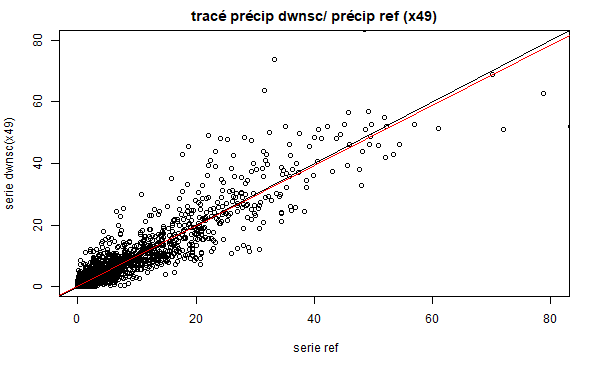
\includegraphics[scale=0.2]{images/pr_3_CDFt_ref.png}
				\end{subfigure}\\
				\begin{subfigure}[b]{0.5\textwidth}
					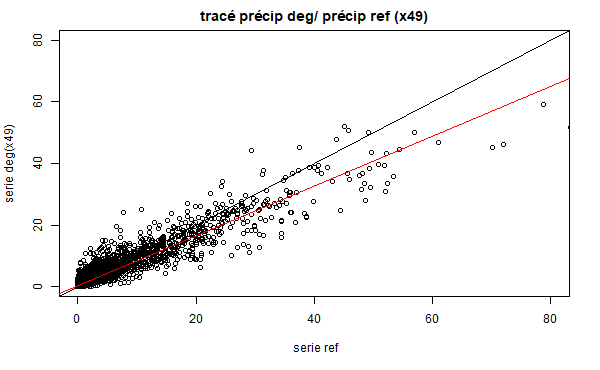
\includegraphics[scale=0.2]{images/pr_3_dg.png}
				\end{subfigure}
			\caption{Tracé des série projetées/ observées}
			\end{figure}
		\end{minipage}
	\end{frame}
	\subsection{Modélisation hydrologique}
		\begin{frame}{Deux modèles pour simuler le fonctionnement hydrologique du Little Washita}
		\begin{minipage}[b]{0.5\linewidth}
				\begin{figure}[H]
					\label{fig-Little Washita 3D}
					\begin{center}
						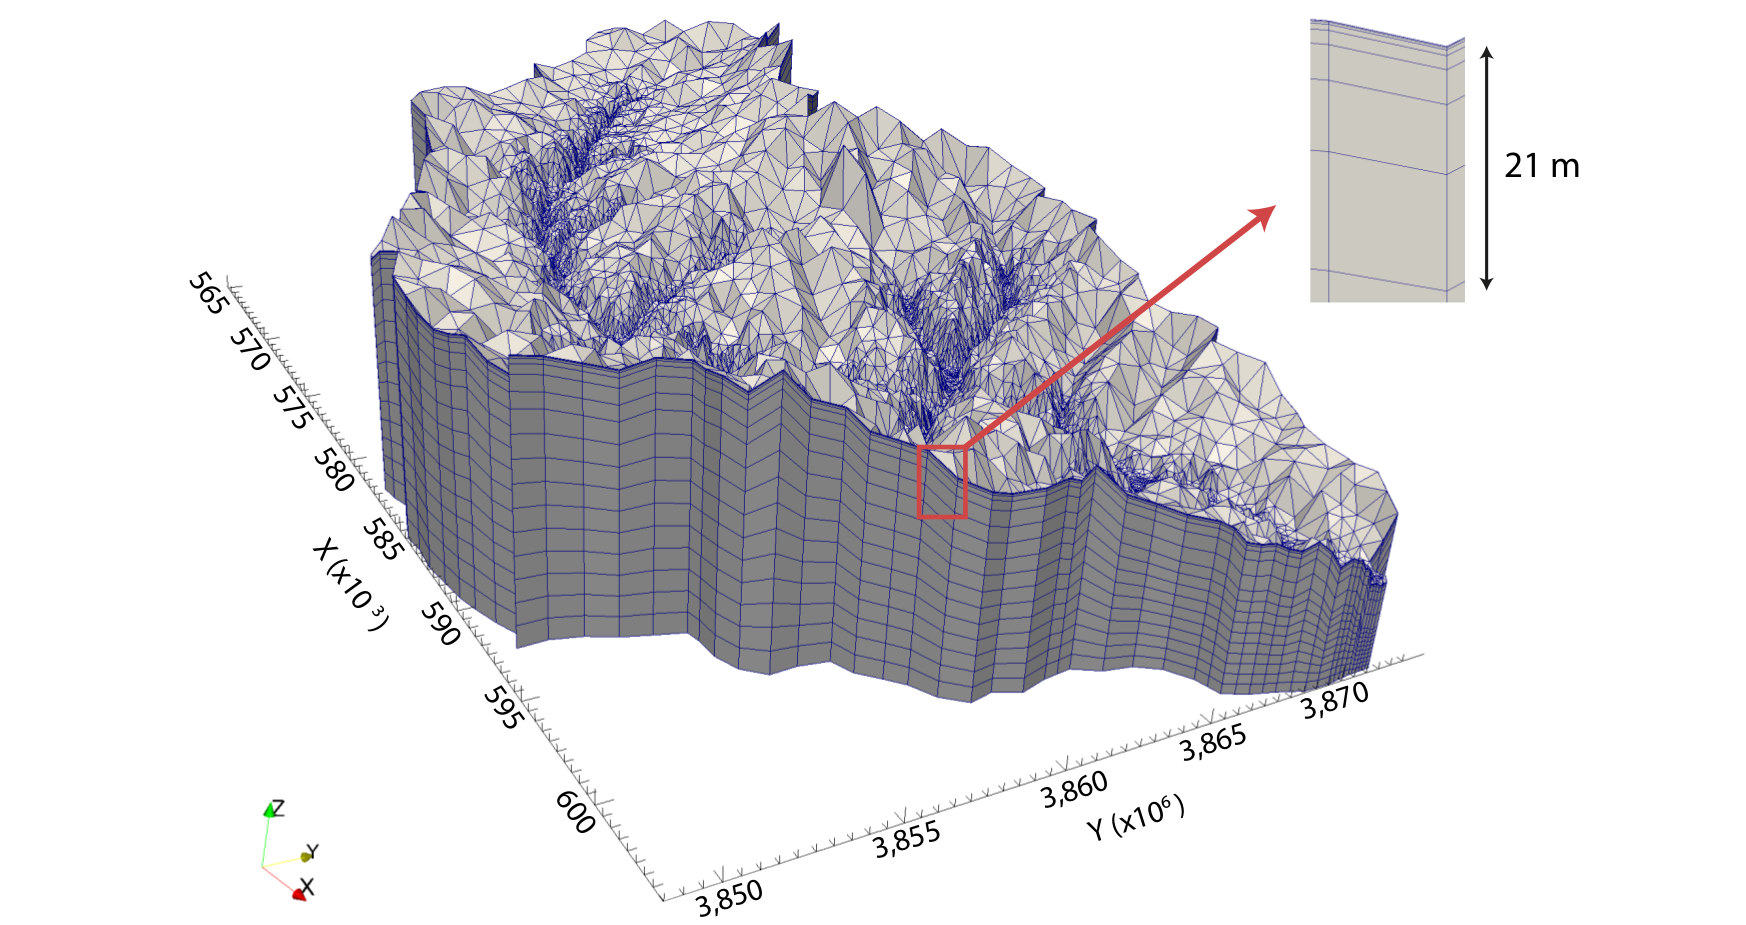
\includegraphics[scale=0.1]{images/little_washita3D.png}
					\end{center}
					\caption{Maillage tridimensionnel du bassin versant du Little Washita}
				\end{figure}
		\end{minipage}\hfill
		\begin{minipage}[b]{0.5\linewidth}
			\begin{figure}[H]
				\label{fig-Little Washita 2D}
				\begin{center}
					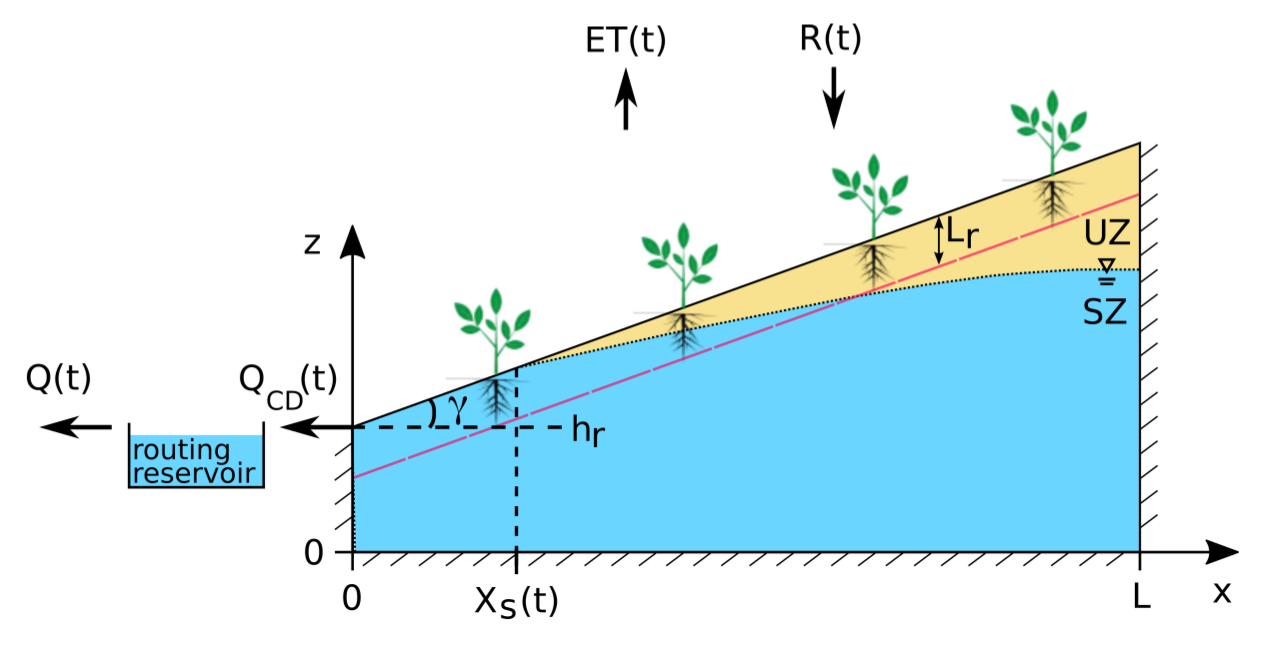
\includegraphics[scale=0.13]{images/upscaling_Little_Washita2D.png}
				\end{center}
				\caption{Upscaling du maillage tridimensionnel du bassin versant du Little Washita (article Fanny)}
			\end{figure}
		\end{minipage}
	\end{frame}
	\subsection{Résultats hydrologiques précipitations débits}
	\begin{frame}
	\begin{figure}
		\begin{center}
			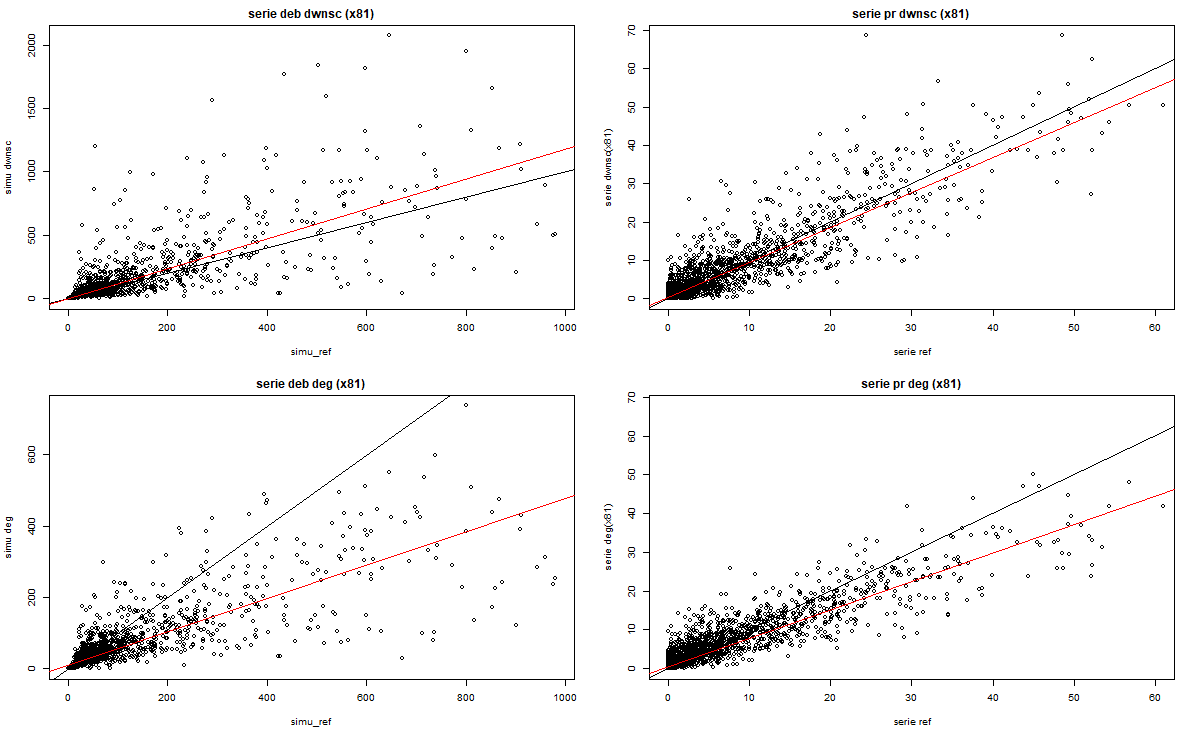
\includegraphics[scale=0.2]{images/multi_comparaison_5.png}
		\end{center}
	\caption{Comparaison débits et précipitations}
	\end{figure}
	\end{frame}

	\subsubsection{Analyse des résultats}
	
	\begin{frame}{Analyses des résultats du downscaling}
		\begin{minipage}[b]{0.5\linewidth}
			\begin{figure}
				\label{fig-res_CVM_CDFt_deb}
				\centering
				\begin{subfigure}[b]{0.5\textwidth}
					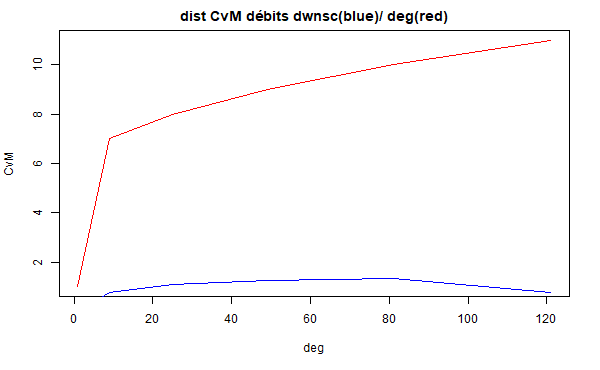
\includegraphics[scale=0.2]{images/Dist_CVM_CDFt_deb.png}
				\end{subfigure}\\
				\begin{subfigure}[b]{0.5\textwidth}
					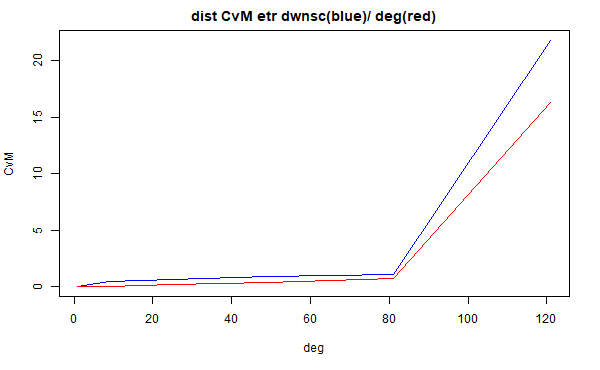
\includegraphics[scale=0.2]{images/Dist_CVM_CDFt_etr.png}
				\end{subfigure}
				\caption{Tracé de la distance de Cramér-von Mises}
			\end{figure}
		\end{minipage}\hfill
		\begin{minipage}[b]{0.5\linewidth}
			\begin{figure}
				\centering 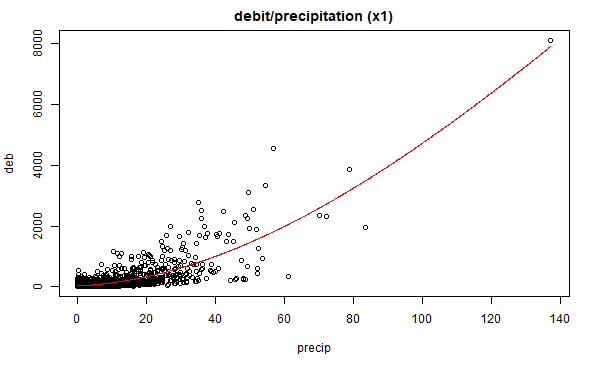
\includegraphics[scale=0.2]{images/deb_rapport_pr_deg1.png}
				\caption{Comportement non linéaire du filtre}
			\end{figure}
		\end{minipage}
	\end{frame}
	
	\subsubsection{Classification de population précipitations-débits}
	
	\begin{frame}{Classifications des données réactives et non réactives aux précipitations}
	\begin{minipage}[b]{0.5\linewidth}
		\begin{figure}[H]
			\label{points}
			\begin{center}
				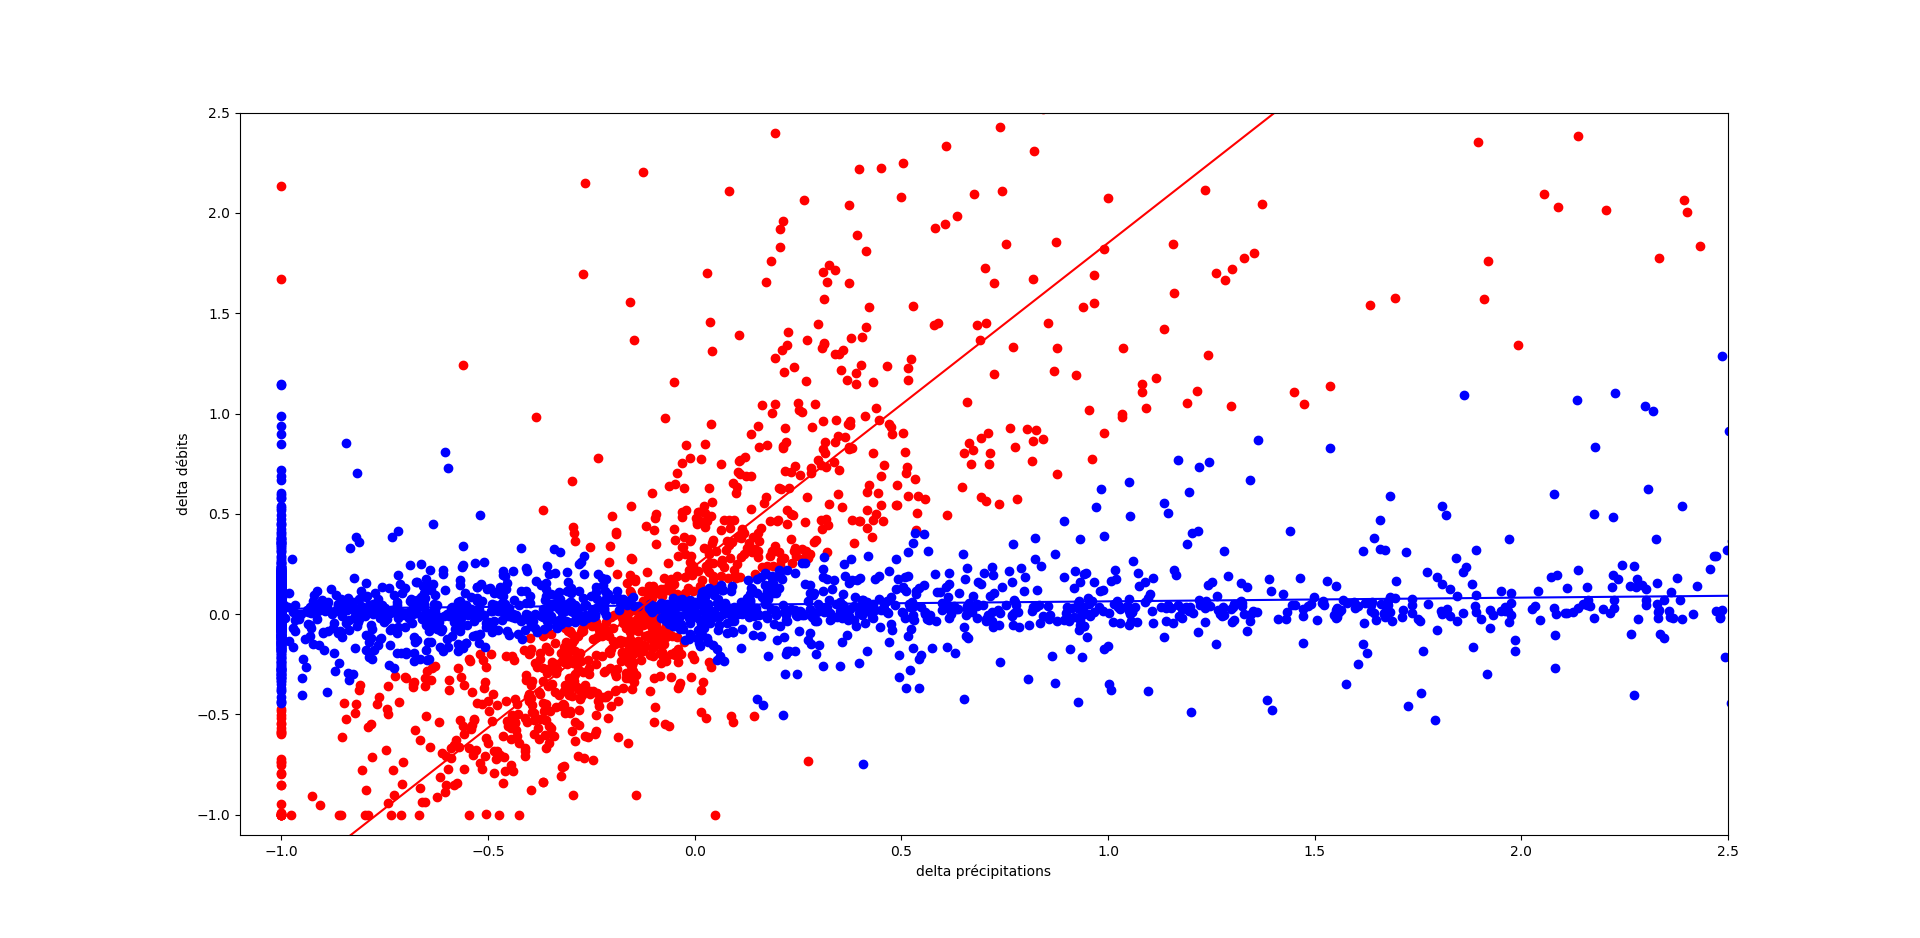
\includegraphics[scale=0.12]{images/classification_deb_pr.png}
				\end{center}
				\caption{Classification des points selon les droites de régression, dégradation $(\times 49)$}
			\end{figure}
		\end{minipage}\hfill
		\begin{minipage}[b]{0.5\linewidth}
			\begin{figure}[H]
				\label{points-2}
				\begin{center}
					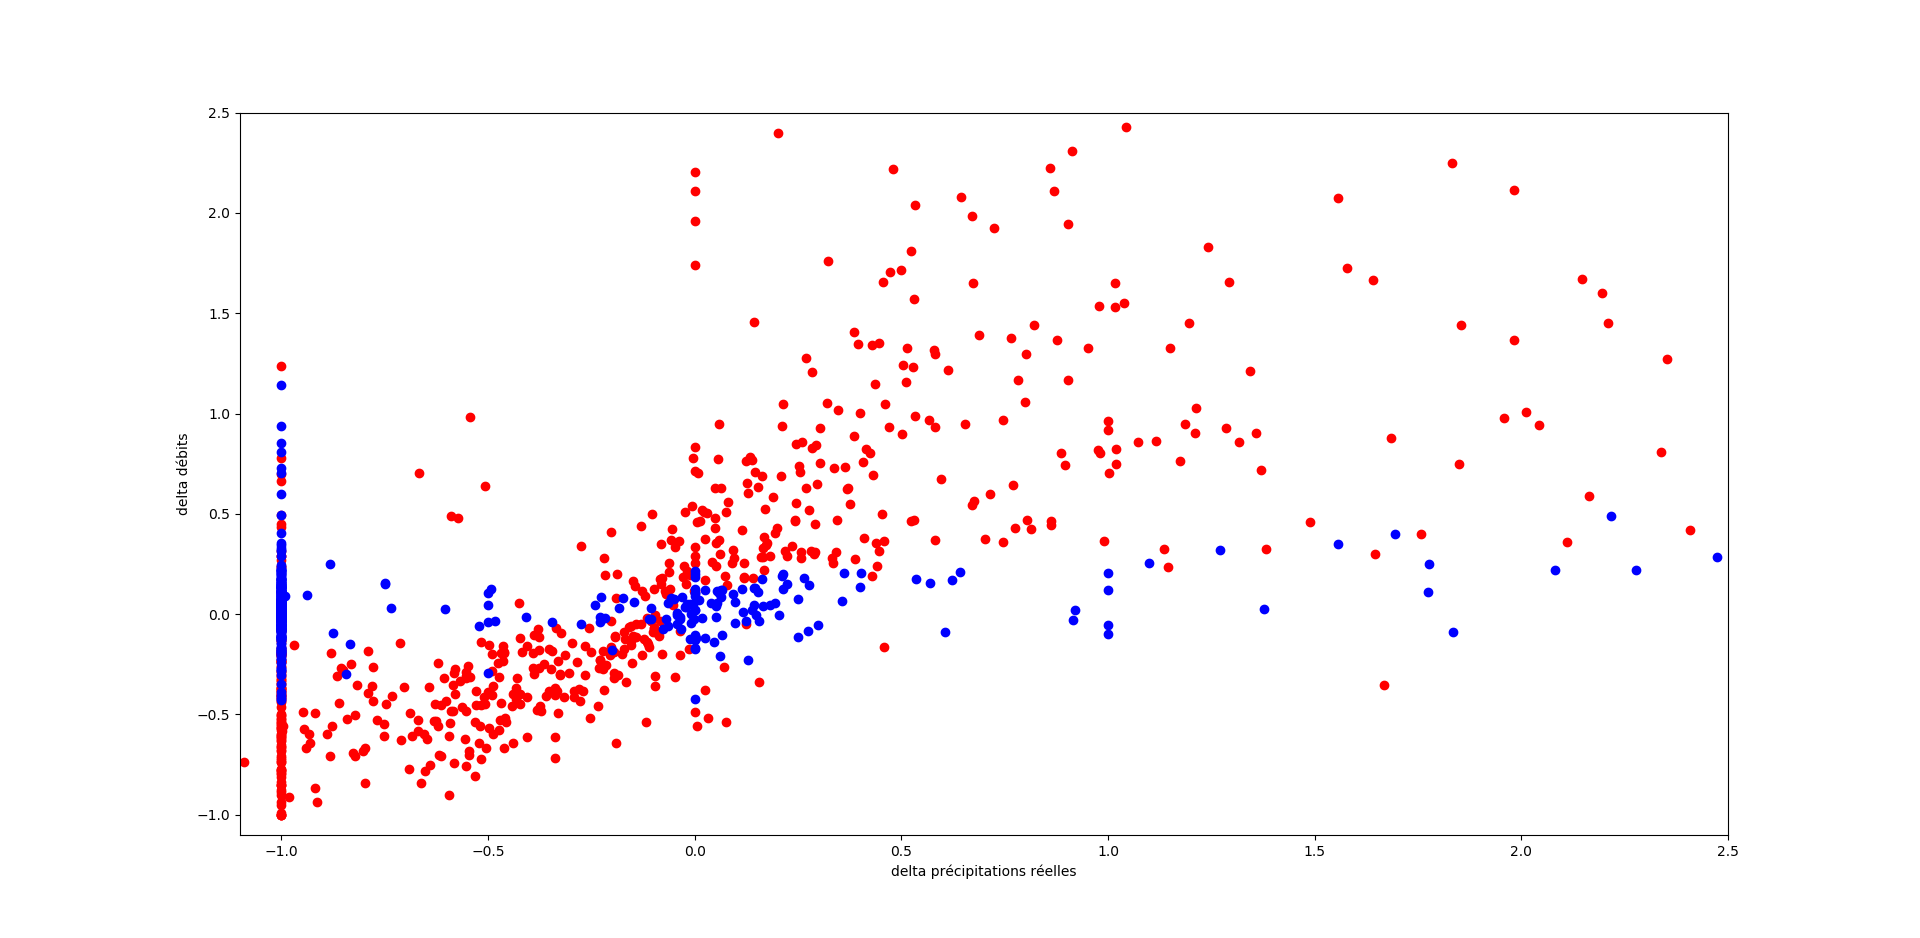
\includegraphics[scale=0.12]{images/classification_deb_prr.png}
					\end{center}
					\caption{Classification pour l'eau entrant dans le sol, dégradation $(\times 49)$}
				\end{figure}
			\end{minipage}
		\end{frame}
	
\end{document}
